%========================= Classe du Document ==========================
\documentclass[a4paper,fleqn]{article}
%============================= Packages ================================
\usepackage[margin=2.5cm]{geometry}
\usepackage[hidelinks]{hyperref}
\usepackage[utf8]{inputenc}
\usepackage[T1]{fontenc}
\usepackage{graphicx}
\usepackage{listings}
\usepackage{amsmath}
\usepackage{amsfonts}
\usepackage{amssymb}
\usepackage[version=4]{mhchem}
\usepackage{stmaryrd}
\usepackage{graphicx}
\usepackage{amssymb}
\usepackage{xcolor}
\setlength{\parindent}{0pt}
%=======================================================================



%========================= Debut du document ===========================
\begin{document}
%=======================================================================


%^^^^^^^^^^^^^^^^^^^^^^^^^^^ Page de Garde ^^^^^^^^^^^^^^^^^^^^^^^^^^^^^
\definecolor{color}{HTML}{FFFFFF}
\pagecolor{color}
\thispagestyle{empty}

\begin{figure}
    \centering
    
\includegraphics[width=8cm]{./uspn.png}
\end{figure}

\vspace{6cm}

\begin{center}
    {\huge \bfseries Connect Four \par}
    
    \vspace{1cm}
    
    \begin{figure}[h]
        \centering
        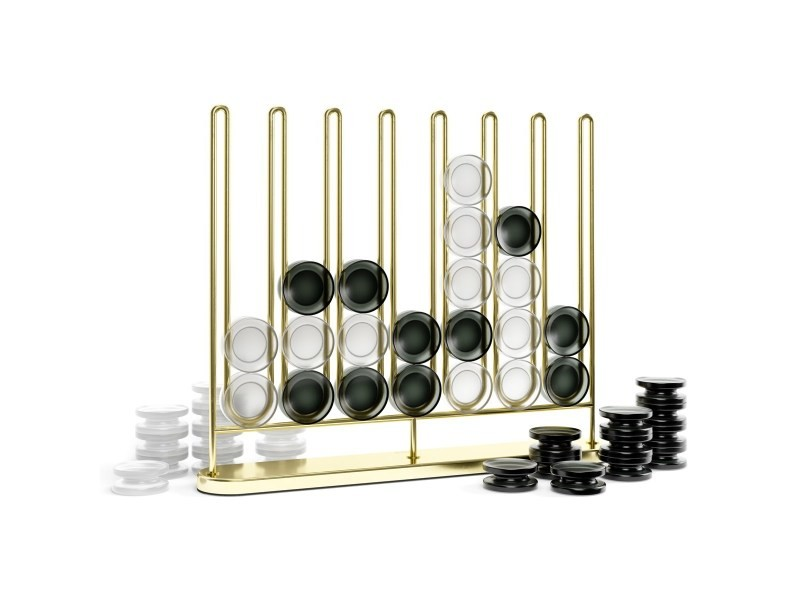
\includegraphics[width=8cm]{./cover.jpeg}
    \end{figure}
    
    \vspace{2cm}
    
    \large Data Structures - J.CHAUSSARD \\
    
    \vspace{1cm}
    
    E.NICOLAS \\
    ING1 INFO - GALILEE INSTITUTE \\
    ethan.bento-nicolas@edu.univ-paris13.fr
    
    \vfill
    
    \today 
    \pagebreak
\end{center}
%^^^^^^^^^^^^^^^^^^^^^^^^^ Fin Page de Garde ^^^^^^^^^^^^^^^^^^^^^^^^^^^

\section*{1 Objectifs et résultats préliminaires}

On souhaite élaborer un algorithme efficace d'inversion d'une matrice $A$ réelle $n \times n$ en utilisant une approche de type "Diviser pour régner". Pour simplifier, on supposera dans ce devoir que $A$ est de taille $2^{k} \times 2^{k}$ avec $k$ entier naturel.

\begin{enumerate}
  \item Montrer que si $A$ est une matrice (réelle) inversible $n \times n$ alors $A^{T} A$ est symétrique et définie positive, i.e. $\forall x \neq 0 \in \Re^{n} x^{T} A^{T} A x>0$.
   \\ On a :  
   \begin{enumerate} 
   \item $ (A^{T} A)^{T} = A^{T} (A^{T})^{T} = A^{T} A$, donc  $A^{T} A$ est symétrique (égale à sa transposée).
   \item $x^{T} A^{T} A x = (Ax)^{T}A x = \|Ax\|_2^2  > 0$ , donc $A^{T} A $ est définie positive.
  \end{enumerate}
    
  \item En déduire que $A^{-1}=\left(A^{T} A\right)^{-1} A^{T}$, et donc que pour calculer l'inverse (si elle existe) d'une matrice quelconque, il suffit de savoir inverser les matrices définies positives. Le coût supplémentaire sera alors constitué d'une transposition et de deux multiplications. \\ On a :  
   \begin{enumerate} 
   \item $ A^{-1} = A^{-1}(A^{T})^{-1}A^{T}= (A^{T} A)^{-1} A^{T}$,  CQFD.
  \end{enumerate}
    

  \item On découpe $A^{T} A$ en blocs de taille $n / 2$. Montrer que $A^{T} A=\left[\begin{array}{cc}B & C^{T} \\ C & D\end{array}\right]$ définie positive équivaut à $S=D-C B^{-1} C^{T}$ définie positive.
  
  \begin{enumerate}
  
 \item Soit $y, z \neq 0 \in \Re^{\frac{n}{2}}$  : \newline 
 $
x^TA^TAx = (y^T z^T)
\begin{bmatrix}
    B & C^{T} \\
    C & D
\end{bmatrix}
\begin{bmatrix}
    y \\
    z
\end{bmatrix}
= (y^T z^T)
\begin{bmatrix}
    By + C^{T}z \\
    Cy + Dz
\end{bmatrix} \newline\newline
= y^TBy + y^TC^Tz + z^TCy + z^TDz \newline\newline
= y^TBy + y^TBB^{-1}C^Tz + z^TCB^{-1}By + z^TCB^{-1}BB^{-1}C^Tz + z^TDz - z^TCB^{-1}C^Tz \newline \newline
= (y + B^{-1}C^Tz)^T B (y + B^{-1}C^Tz) + z^T (D - CB^{-1}C^T)z
$
 
 \item Or, soit y un vecteur non nul tel que $y = -B^{-1}C^Tz$ alors : \newline $x^TA^TAx > 0 \iff z^TSz > 0$.

\end{enumerate}
    

  \item En déduire que $(A^{T} A)^{-1} = \left[\begin{array}{cc}B^{-1}+B^{-1} C^{T} S^{-1} C B^{-1} & -B^{-1} C^{T} S^{-1} \\ -S^{-1} C B^{-1} & S^{-1}\end{array}\right]$ \newline
  
 On passe par la méthode "barbare" en calculant $A^{T} A(A^{T} A)^{-1}$ : \newline $\left[\begin{array}{cc}B & C^{T} \\ C & D\end{array}\right] \left[\begin{array}{cc}B^{-1}+B^{-1} C^{T} S^{-1} C B^{-1} & -B^{-1} C^{T} S^{-1} \\ -S^{-1} C B^{-1} & S^{-1}\end{array}\right] $
   \begin{enumerate}
  
  \item  En haut à gauche : \newline $B(B^{-1}+B^{-1} C^{T} S^{-1} C B^{-1})  - C^{T} (S^{-1} C B^{-1})) = I_\frac{n}{2}$
  \item  En haut à droite : \newline $B(-B^{-1} C^{T} S^{-1}) + C^{T}S^{-1} =  0$ 
  \item  En bas à gauche : \newline $C(B^{-1}+B^{-1} C^{T} S^{-1} C B^{-1})  - D(S^{-1} C B^{-1}))  \newline = CB^{-1}+CB^{-1} C^{T} S^{-1} C B^{-1}  - DS^{-1} C B^{-1} \newline = CB^{-1} + (CB^{-1}C^{T}S^{-1} - DS^{-1}) C B^{-1} = 0 \newline = CB^{-1} + ((CB^{-1}C^{T} - D)S^{-1}) C B^{-1} \newline =  CB^{-1} + (-SS^{-1}) C B^{-1} \newline = 0$
  \item  En bas à droite : \newline $C(-B^{-1} C^{T} S^{-1}) + DS^{-1} =  (-CB^{-1} C^{T} + D)S^{-1} = SS^{-1} = I_\frac{n}{2}$
  
  On retrouve bien une matrice identité de taille $n\times n$.
  

\end{enumerate}

\end{enumerate}

\break 
\section*{2 Algorithme et analyse de sa complexité}
On considère alors l'algorithme suivant pour calculer $A^{-1}$.

\begin{enumerate}
  \item Calculer $A^{T} A$ (multiplication standard ou algorithme de Strassen).

  \item Calculer récursivement l'inverse de $A^{T} A$ en découpant la matrice en quatre sousmatrices de taille $2^{k-1} \times 2^{k-1}$ et en relançant la fonction pour calculer les inverses de $B$ et de $S$. Lorsque $B$ et $S$ sont de taille $1 \times 1$, il suffit de prendre les inverses des deux nombres réels (on peut détecter que la matrice est non inversible si on trouve $B=0$ ou $S=0$ ). A chaque retour de récursion, utiliser la formule de la question (4) de la section précédente pour calculer la matrice inverse.

  \item Calculer $A^{-1}=\left(A^{T} A\right)^{-1} A^{T}$ pour obtenir l'inverse de $A$, puis afficher le résultat.

\end{enumerate}

Lors de l'étape (2) pour obtenir $\left(A^{T} A\right)^{-1}$ on calcule dans l'ordre suivant les différents éléments : $B^{-1}, C B^{-1}$ et sa transposée $B^{-1} C^{T}, S, S^{-1}, S^{-1} C B^{-1}$ et sa transposée, et enfin $B^{-1} C^{T} S^{-1} C B^{-1}$ et $B^{-1}+B^{-1} C^{T} S^{-1} C B^{-1}$. \newline

 Calcul de la complexité :
\begin{itemize} 

\item 2 appels récursifs avec des matrices  $\frac{n}{2} \times \frac{n}{2}$ donc $C(n) = 2C\left(\frac{n}{2}\right) + \beta$.

\item  On a $\beta$ : 4 multiplications  pour les sous matrices de taille $\frac{n}{2}$) en $O(n^3)$ en standard ou $O(n^{\log_2 7})$ pour Strassen, 1 addition en $O(n^2)$, 3 soustractions dont 2 à 0 (même chose qu'une multiplication par le scalaire -1 en complexité) en $O(n^2)$, 2 transpositions en $O(n^2)$. On a également les découpages / recollages de matrices sui sont en $O(n^2)$ (on traverse les éléments de la matrice que l'on range en fonction de leur indice).

\item Donc, $C(n) = 2C\left(\frac{n}{2}\right) + 4O(n^3) + 8O(n^2) = 2C\left(\frac{n}{2}\right) + O(n^3)$, d'après le $Master$ $Theorem$, on a $3 > \log_2 2 = 1$ donc la complexité est en $O(n^3)$ ou $O(n^{\log_2 7})$ en utilisant Strassen. On remarque que l'inversion de matrices se résume à la complexité de la multiplication utilisée.

\end{itemize}

\break
\section*{3 Implémentation}
Problèmes rencontrés lors de l'implémentation et analyse :

\begin{enumerate}
  \item Problèmes de récursion, trop d'appels sur le stack (pile des appels récursifs des fonctions) introduisent une moins bonne efficacité. En effet, Strassen est moins bon que la multiplication standard avec les récursions alors que la complexité est sensée être meilleur. Cela induit une difficulté intéressante dans le sens que l'implémentation effectué ne reflète pas forcément la complexité que l'on peut calculer. Le moyen de contourner les ralentissements seraient d'appliquer les fonctions à une matrice globale et ou l'on joue avec les indices des sous-matrices. Les appels récursifs seraient un changement d'indice et le rappel des fonctions sur ces nouveaux indices. (Voir Fig. 1, 2 et Table 1).
  

  \item Problème de l'inversion (voir test de la matrice de 128). On se rend compte que lors de l'inversion des nombres, l'approximation faite va obligatoirement amené de la propagation d'erreurs lors de calculs (encore plus avec Strassen vu le nombre de sous-produit effectués). On voit qu'il y a des erreurs minsucules de l'ordre de $10^-7$. Ainsi, la réflexion sur la représentation des nombres et de comment l'inversion de nombre peut être faite pour ne perdre aucune information. L'idée pourrait être de donner les valeurs en fraction irréductible ou d'utiliser des méthodes de raffinement comme la méthode de Newton-Raphson en utilisant des valeurs précises (cf. "Fast inverted square root" and https://pvk.ca/Blog/LowLevel/software-reciprocal.html).

  \item Cependant, dans l'utilisation de matrices raisonnables et bien conditionnés, le codage à froid de l'algorithme fonctionne même si les performances ne sont pas au rendez-vous (notamment pour Strassen). Plus de temps et de moyens (articles de recherches sur l'inversion de double en informatique) permettrait d'améliorer significativement les performances et la taille des matrices en entrée. \end{enumerate}
 
 
\section{4 Tests}

Pour la matrice de 128 fournie dans les données on a : 
\begin{enumerate}

\item Matrice Originale :

[[2.30000000 2.90000000 1.70000000...2.00000000 0.80000000 0.30000000]
[1.50000000 1.00000000 0.20000000...2.10000000 0.40000000 0.30000000]
[2.30000000 2.30000000 2.20000000...2.20000000 2.90000000 1.20000000]
 
...

 [1.30000000 2.10000000 2.60000000...2.70000000 0.50000000 2.80000000]
 [2.10000000 1.10000000 0.10000000...2.70000000 1.60000000 1.60000000]
 [1.30000000 2.70000000 2.30000000...0.90000000 0.80000000 0.90000000]]
\item Inverse :

[[-0.45851911 -0.53444141 2.85526750...4.47284235 -2.20848939 4.19048636]
[0.40250065 0.34154857 -2.55377462...-3.89081042 2.00200523 -3.73161581]
[2.21507473 2.37101363 -13.32954725...-20.59551802 10.45334918 -19.54867214]
 
...

[-1.64574242 -1.75513486 10.27559414...15.86334813 -8.02919982 15.00229281]
[-0.01866825 -0.01736101 0.20034185...0.39654035 -0.16978280 0.38588121]
[-1.29892230 -1.23564963 7.23799216...11.04957259 -5.68094990 10.50274516]]
 
\item Produit Inverse/Matrice (Identité) :

[[0.99999998 -0.00000003 -0.00000003...-0.00000001 -0.00000000 0.00000000]
[0.00000002 1.00000003 0.00000003...0.00000001 0.00000000 -0.00000000]
[0.00000011 0.00000014 1.00000013...0.00000002 0.00000001 -0.00000001]
 
...

[-0.00000009 -0.00000011 -0.00000010...0.99999998 -0.00000001 0.00000000]
[-0.00000000 -0.00000000 -0.00000000...0.00000000 1.00000000 0.00000000]
[-0.00000006 -0.00000007 -0.00000007...-0.00000001 -0.00000000 1.00000001]]

\item Inverse trouvé avec la bibliothèque numpy :

 [[-4.58519042e-01 -5.34441340e-01  2.85526711e+00 ...  4.47284178e+00
  -2.20848909e+00  4.19048580e+00]
 [ 4.02500586e-01  3.41548507e-01 -2.55377428e+00 ... -3.89080991e+00
   2.00200497e+00 -3.73161531e+00]
 [ 2.21507441e+00  2.37101331e+00 -1.33295454e+01 ... -2.05955153e+01
   1.04533478e+01 -1.95486695e+01]
   
 ...
 
 [-1.64574218e+00 -1.75513461e+00  1.02755928e+01 ...  1.58633461e+01
  -8.02919874e+00  1.50022908e+01]
 [-1.86682480e-02 -1.73609992e-02  2.00341815e-01 ...  3.96540300e-01
  -1.69782774e-01  3.85881164e-01]
 [-1.29892213e+00 -1.23564946e+00  7.23799119e+00 ...  1.10495711e+01
  -5.68094914e+00  1.05027437e+01]]

\break
 
\section*{5 Figures}
\begin{table}[htbp]
  \centering
  \begin{tabular}{|c|c|c|c|}
    \hline
    Taille & Strassen & Multiplication standard \\
    \hline
    2 & 0.000005 & 0.000014 \\
    4 & 0.000057 & 0.000018 \\
    8 & 0.000430 & 0.000049 \\
    16 & 0.003035 & 0.000116 \\
    32 & 0.012115 & 0.000240 \\
    64 & 0.060335 & 0.000401 \\
    128 & 0.438345 & 0.001464 \\
    256 & 3.149275 & 0.011411 \\
    512 & 21.937766 & 0.101327 \\
    \hline
  \end{tabular}
    \caption{Temps d'exécution pour différentes tailles de matrices}
\end{table}


\end{enumerate}

\end{document}